%!TEX root = ../../thesis.tex

\graphicspath{{Chapters/conclusion/figures/}}

\chapter{Conclusion}
This thesis first covered the mechanics of neural networks: their fundamental construction, how neurons compose
to form more complex functions, and how they learn. Next was the exploration of how to operate these networks, starting
with how to train them, then how to identify and diagnose potential issues like over-fitting, and then some
more advanced techniques to increase their performance. After that, more specialized
components specifically used in the construction of convolution neural networks were discussed, as were the image datasets used to
evaluate this class of model. The final pieces of the rudiments were the practicalities of neural network research,
specifically the hardware and software frameworks necessary for efficient work.

With the fundamentals covered, the world of state-of-the-art convolutional neural networks was entered,
starting with the networks like AlexNet, Inception, and ResNet that were formative in modern architecture design. From there,
the first neural architecture search techniques like NAS-RL and Neuroevolution were examined, ones that
demonstrated that automated methods could indeed build competitive architectures. However, these first approaches
used huge amounts of computational power, and were impractical for real-world uses. This brought us to the second
generation of NAS algorithms like ENAS and Regularized Evolution, that sought to optimize these earlier algorithms
and reduce their costs. This drive towards efficiency led us to differentiable approaches like DARTS and ProxylessNAS,
that made use of gradient descent to perform both architecture search and model training, an elegant and conceptually compact
solution to the NAS problem. However, these results could not be discussed without also exploring the criticisms that plagued all of these approaches:
a random search policy in their search space often performed equally well as these intelligent methods. This set the stage
for the research questions explored in this work.
\vspace{-1em}
\section{Search Space Expansions}
My hypothesis as to why random search performed so well as compared to intelligent search concerned search space
design bias; that the extensive research into manual architecture design over common benchmark datasets like CIFAR and
ImageNet contaminated how NAS researchers built their search spaces. These `constricted' search spaces were so shaped
by this contaminatory bias as to exclusively contain good models, and therefore, NAS or random search policies would
perform well regardless of their decisions.
\vspace{-1em}
\subsection{BonsaiNet}
Testing this hypothesis first entailed building the Bonsai search space. By allowing each edge in the models to be
multi-path (i.e, contain multiple mixed operations), expanding the potential cellular inputs to be any possible mixture of
prior cell outputs, and removing the restriction of cellular homogeneity, the search space expanded by a factor of
roughly $10^{200}$ as compared to the constricted spaces used in~\cite{li2019} or~\cite{yu2019}. While
much larger, the Bonsai space is also crucially a superset of those constricted spaces; all the good architectures
are still present while dramatically increasing the probability for bad architectures to exist. Indeed, this had the desired
effect of lowering the average quality of randomly selected models, with a random network from the Bonsai search space
scoring a 95.19\% accuracy on CIFAR-10, while a random model in the constricted space scored a 96.48\%. With a lowered
random search benchmark, NAS has more room by which to demonstrate its abilities, if it can truly discern quality models
within a search space.

However, the size of the Bonsai search space presented its own challenges to NAS, as many of the design restrictions
in the constricted space are put in place due to hardware restrictions like VRAM space. To perform NAS in the Bonsai search
space, an algorithm needed to be designed that could perform effectively. This algorithm became BonsaiNet, which
uses differentiable pruners and the concept of model compression to iteratively build networks. First, BonsaiNet
divides a model supernet into roughly even `sections' that are all small enough to fit uncompressed into the available
GPU space. BonsaiNet then iteratively builds itself by instantiating a model section, then uses the differentiable pruners
within to compress the model until the next section can be appended. This process cycles until the model has grown to the
full size as specified in the configuration, at which point it can train normally.

This process provides many advantages, namely that models derived from very VRAM-expensive supernets can be trained
within smaller VRAM footprints. This is evidenced by the experiments within Section~\ref{sect:supernetevaluation},
which found that BonsaiNet only needed 10.5 GB of VRAM to identify an optimal subnet within a 15 GB supernet. While
`only' a 30\% space savings, it marks the difference between being able to run the network on an NVidia 1080Ti and
needing a more expensive, more spacious GPU. Additionally, the found network was only minimally less accurate than
one isolated directly from pruning the full supernet while requiring a final
VRAM footprint of only 7.39 GB, which is small enough to fit on the majority of consumer GPUs.  Therefore,
in a search space that contained models up 15 GB large, BonsaiNet was able to find one that was only 7.39 GB
yet offered equal accuracy performance to the largest models. In this sense,
BonsaiNet is exceptionally capable at finding optimal, efficient models within search spaces that would
ordinarily be well outside the spatial capabilities of the available hardware.

BonsaiNet's raw capabilities aside, it also consistently found models that had significant accuracy improvements
over random search: the average small-cell BonsaiNet model scored a 96.65\% test accuracy over CIFAR-10. This is exactly
in line with performance of NAS algorithms in the constricted space that were presented in~\cite{yu2019}, which on average
found models of around 96.55\% test accuracy. Therefore, despite the average quality of models in the space decreasing,
BonsaiNet was still able to identify the good models still present. The expanded search space did not seem to hinder
the calibre of BonsaiNet's discovered models either, as they are comparable to the good models that were being discovered
in the original constricted space. This is made explicitly clear in Figure~\ref{fig:nas_v_random}:

\begin{figure}[ht!]
    \centering
  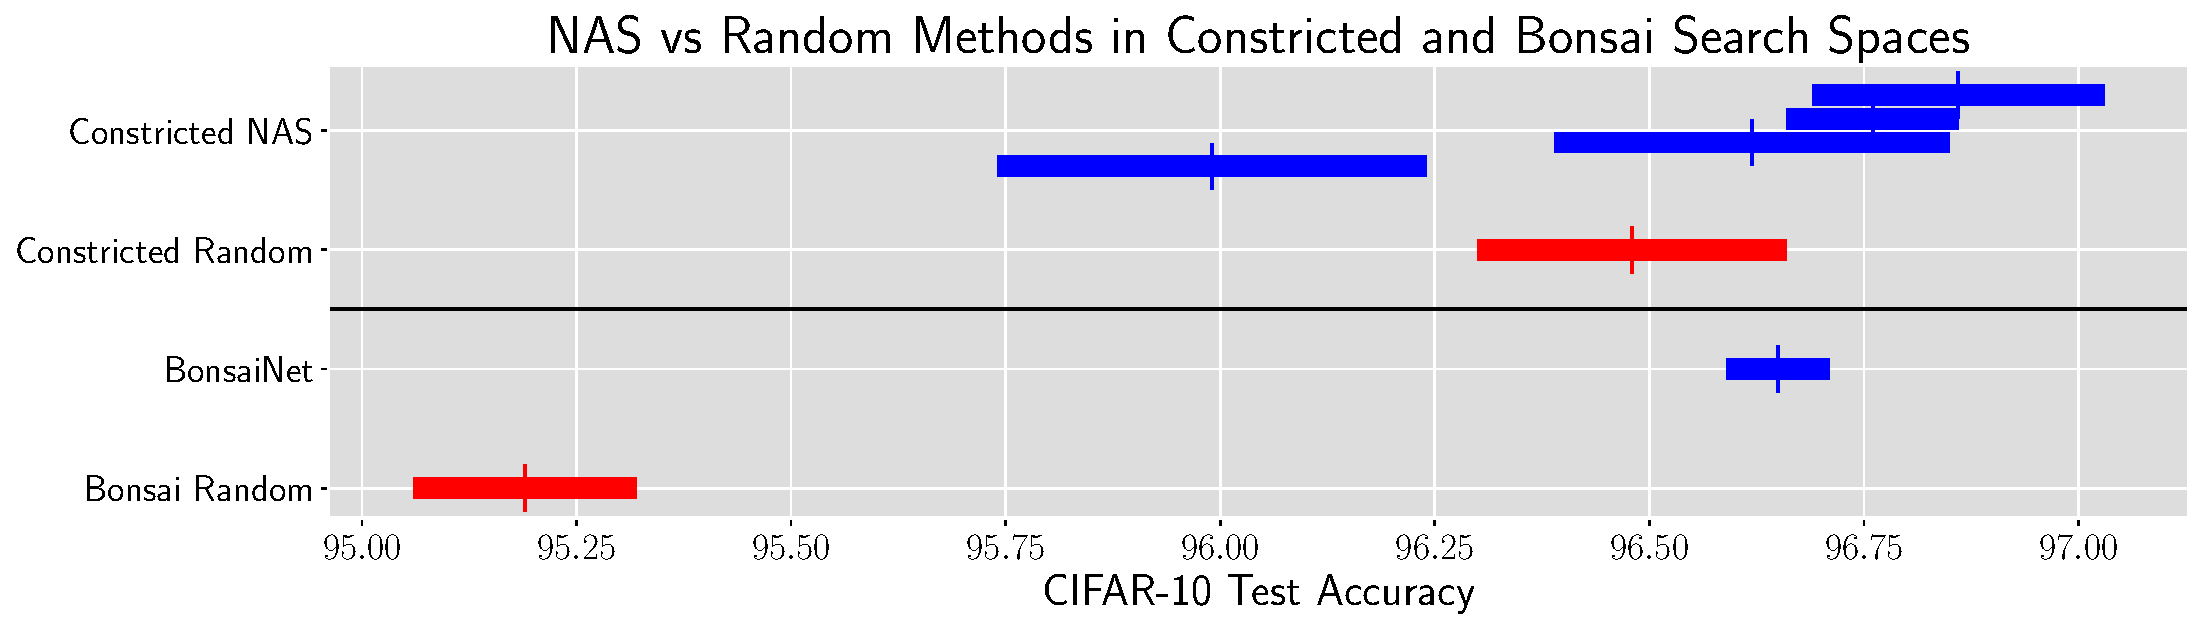
\includegraphics[width=\textwidth]{nas_v_random}
    \caption[Random and NAS models'
    performances on the constricted \citeauthor{yu2019} and Bonsai search spaces]{Random and NAS models'
    performances on the constricted \citeauthor{yu2019} and Bonsai search spaces. From top to bottom, the
    constricted NAS entries correspond to NAO, ENAS, DARTS, and BayesNAS respectively.}
    \label{fig:nas_v_random}
\end{figure}

This indicates that the random search hypothesis was indeed correct: random search only compares well to NAS when
the search space contains exclusively good models; its comparable ability is merely an illusion caused by an over-constricted
search space. In a space with greater performance variance, random search suffers while NAS is still able to identify
the high-performance models.

\subsection{SpiderNet}
While BonsaiNet demonstrates NAS' ability to differentiate between good and bad models in search spaces containing models
of more variable accuracies, SpiderNet revealed a different virtue that NAS can possess. SpiderNet takes the expanded
search space of BonsaiNet to its logical extreme, instead operating in an infinite search space bound only by available search
time. By nature of its mutations and unbounded search space, SpiderNet produces very complex, organic-looking
models as compared to BonsaiNet (compare Figure~\ref{fig:bonsai_cell} to Figure~\ref{fig:spider_rand0_example}
for a clear example of this). Specifically, SpiderNet defines a triangular mutation, which adds a new node and two
edges to an existing edge to create a new, triangularly connected system. By performing these mutations over edges
in a model, the model can be dynamically grown. Differentiable pruners lying along these edges can then
conversely prune the model as desired, meaning models exist in a constantly growing and shrinking search space.
Different metrics were explored to guide where these mutations should occur, and found that performing mutations on edges
with a minimum pruner variance or optimal NTK-LRC scores was best. Interestingly, traversing this space via random mutation
often produces networks that were nearly as accurate as those produced by minimum-variance or NTK-LRC guided mutations.

However, the models produced by the guided mutations were much more time and parameter efficient than the randomly
generated models. Often, the few hours that a guided-mutation search took were made up for during training, as the much
more time-efficient model could train significantly faster than the random models. This erodes one of random search's
predominant advantage: its lack of search cost. This is best demonstrated in Table~\ref{tab:spider_rand2}; the guided
mutations took 5.4 hours to produce a network as compared to the functionally zero cost of producing a network at random.
However, the guided mutation model took 12 hours less to train than the random one, meaning the end-to-end time costs
were around 6.5 hours cheaper. Additionally, the guided mutation model used half as many parameters and scored 0.1\% percentage
points higher accuracy than the random model.

Therefore, if NAS can be more parameter efficient and outright faster end-to-end than random search, why does it matter
that random search can produce models that are \textit{almost} as good? If random search cannot outperform NAS on raw accuracy,
the only reason to use it would be its search cost advantage. However, when considering the full context of how these
networks are used, the search cost constitutes a tiny fraction of the total time required to produce a fully trained model,
around 7\% in this example. Conceding some time in this 7\% to prioritize efficiency in the remaining
93\% is more than worth it. Training and evaluation costs of the networks produced by NAS is significantly more relevant
to the practical costs of NAS than search cost, considering
that cloud providers bill hourly. Perhaps the focus on search-time seen in literature is a holdover from the era of algorithms like NAS-RL that
needed 61 years of search time to produce an architecture, in which case you might be able to get results faster by
training a random network with pen and paper, but this is no longer the case. Search costs are minimal compared to training costs,
and thus I argue that purely accuracy-based comparisons to random search are obfuscating the true utility of NAS.

\vspace{-1em}
\section{Minimizing Configuration}
Finally, as a by-product of the work on BonsaiNet and research into other NAS methods, I noticed a troubling problem
with most NAS algorithms. Due to the configurational requirements (for example, needing to specify node count and
depth in BonsaiNet), there is still a massive amount of manual design necessary when working with NAS. While
BonsaiNet was shown to be fairly robust over configuration changes, producing competitive models across the various
small and large cell domains, a significant amount of time was spent tweaking these configurations in hopes of
producing even better models. This is exactly contrary to the goals of NAS, that is, to minimize the amount of tinkering
necessary in the design of neural networks. As such, two developments that are presented in this thesis provide proof-of-concept
towards minimizing the configurational options necessary of NAS algorithms.

First is the large-cell concept that BonsaiNet can be configured to use and SpiderNet exclusively uses. Here, a series
of small cells consisting of stacking combinations of normal and reduction cells are replaced by a few reduction cells,
of equal number to the total number of desired reductions in the cell. By sufficiently increasing the size of these reduction cells,
all possible stacks of the ubiquitous $N$-normal-cells-plus-a-reduction pattern are simply subgraphs of the large
reduction cell. This means that rather than having to specify the overall cellular structure of a model, i.e, how many
normal cells should be placed before and after each reduction cell, one can just specify the total number of reductions.
This reduces a two-dimensional configuration space ($N_{normal} \times N_{reduction}$) to a single value, $N_{reduction}$.

Second is SpiderNet's ability to shape itself into an appropriate size as it sees fit. Since its starting architecture is
defined simply by the smallest possible initial state, it does not need any configuration as to cellular size. As such,
this eliminates any need to specify cellular node counts or depths, as both values dynamically change per-cell as
the model mutates.

The difference these changes make can easily be seen by a thought-experiment. Imagine a NAS method that
takes 50 GPU hours to produce a fully trained model, and each of its configurational
parameters has three possible values. If neither large-cells nor a self-shaping method are used, there are
four dimensions of configuration: $\left(N_{normal}
\times N_{reduction} \times N_{nodes} \times {N_{depth}}\right)$. In this case, this simple 3 value grid search would cost
4,050 GPU hours to complete, just under 169 GPU days. Meanwhile, a NAS method with large-cells and self-shaping needs just
a single value, $N_{reduction}$, which would mean the grid search would take just six GPU days.

SpiderNet is by no means entirely free of configuration options; it still requires the user to specify batch size,
initial channel size, and of course reduction count. That said, it drastically reduces the amount of tuning necessary to
produce good results, and as such is an excellent step towards the ideal of a truly configuration-free NAS algorithm.
\vspace{-1em}
\section{Final Thoughts}
The results presented here all bode very well for the real-world applicability of NAS. In practice, NAS would be best applied to novel problems,
ones without extensive research into their best practices. The whole idea of NAS is to eliminate the need for such
research in the first place. In such cases, biasing the NAS search space towards good results is impossible, at least
not deliberately. It can be assumed that these `uninformed' search spaces would likely contain both good and bad models,
as what constitutes good and bad cannot be confidently known at the outset. The work in this thesis shows that NAS is
capable of differentiating between said good models and bad models, and is thus well-suited to exactly this application
to novel problems. Furthermore, if designed such as to prioritize this, NAS algorithms can produce highly time and
parameter efficient models, meaning that using NAS can not only reduce development costs,
but also long-term deployment costs. Finally, the work on a minimally-configured NAS algorithm demonstrates that
NAS can define its own architectural requirements for success which minimizes the time required to tune these algorithms.
As such, BonsaiNet and SpiderNet demonstrate the greatest attributes and potential of NAS: it can be an out-of-the-box
solution that identifies fast, efficient, and powerful neural networks at a cost accessible to all.